\RequirePackage{plautopatch}
\documentclass[dvipdfmx,12pt,aspectratio=169]{beamer}
\usepackage{bxdpx-beamer} % dvipdfmxなので必要

% === Required Packages ===
\usepackage{ascmac}
\usepackage[table]{xcolor}        % \rowcolors, \cellcolor
\usepackage{array}                % \newcolumntype
\usepackage{adjustbox}            % \begin{adjustbox}
\usepackage[linesnumbered, ruled, vlined]{algorithm2e}    % \begin{algorithm2e}
\usepackage{amsmath}              % \begin{align*}
\usepackage{amssymb}              % \mathbb{A}
\usepackage{amsthm}               % \newtheorem
\usepackage{bm,bbm}               % \bm{A}, \bbm{1}
\usepackage{booktabs}             % \toprule, \midrule, \bottomrule
\usepackage{cancel}               % \cancel{a}, \bcancel{b}, \xcancel{c}
\usepackage{enumitem}
\usepackage{fancybox}             % \doublebox, \shadowbox
\usepackage{hyperref}             % \href{URL}{text}
\usepackage{ifthen}               % \ifthenelse
\usepackage{lipsum}               % \lipsum
\usepackage{makecell}             % \makecell{L1\L2}
\usepackage{mathrsfs}             % \mathscr{A}
\usepackage{mathtools}            % \mathrlap
\usepackage{multirow}             % \multirow
\usepackage{optidef}              % \begin{mini*}{x}{f(x)}{}{}
\usepackage{orcidlink}            % \orcidlink
\usepackage{physics}              % \qty, \norm, \abs
\usepackage{subcaption}           % \captionsetup
\usepackage{subfiles}             % \subfile{file}
\usepackage{thm-restate}          % \begin{restatable}{theorem}{thm}
\usepackage{tikz}                 % \begin{tikzpicture}
\usepackage{xparse}               % \NewDocumentCommand
\usepackage{mwe}
\usepackage[sort&compress]{natbib}

\usepackage{caption}
\captionsetup[table]{justification=centering}
\captionsetup[figure]{justification=centering}

\definecolor{cA}{HTML}{0072BD}
\definecolor{cB}{HTML}{EDB120}
\definecolor{cC}{HTML}{77AC30}
\definecolor{cD}{HTML}{D95319}
\definecolor{cE}{HTML}{7E2F8E}
\definecolor{tabA}{HTML}{1f77b4}
\definecolor{tabB}{HTML}{ff7f0e}
\definecolor{tabC}{HTML}{2ca02c}
\definecolor{tabD}{HTML}{d62728}
\definecolor{tabE}{HTML}{9467bd}

\newcommand{\red}[1]{\textcolor{red}{#1}}
\newcommand{\blue}[1]{\textcolor{blue}{#1}}
\newcommand{\cyan}[1]{\textcolor{cyan}{#1}}
\newcommand{\gray}[1]{\textcolor{gray}{#1}}
\newcommand{\green}[1]{\textcolor{green}{#1}}
\newcommand{\brown}[1]{\textcolor{brown}{#1}}
\newcommand{\black}[1]{\textcolor{black}{#1}}
\newcommand{\orange}[1]{\textcolor{orange}{#1}}
\newcommand{\purple}[1]{\textcolor{purple}{#1}}
\newcommand{\st}{\text{ s.t. }}
\newcommand{\Img}[1]{\mathrm{Im}\qty(#1)}
\newcommand{\Ker}[1]{\mathrm{Ker}\qty(#1)}
\newcommand{\Supp}[1]{\mathrm{supp}\qty(#1)}
\newcommand{\Rank}[1]{\mathrm{rank}\qty(#1)}
\newcommand{\floor}[1]{\left\lfloor #1 \right\rfloor}
\newcommand{\ceil}[1]{\left\lceil #1 \right\rceil}
% C++ (https://tex.stackexchange.com/questions/4302/prettiest-way-to-typeset-c-cplusplus)
\newcommand{\Cpp}{C\nolinebreak[4]\hspace{-.05em}\raisebox{.4ex}{\relsize{-3}{\textbf{++}}}}
% https://tex.stackexchange.com/questions/28836/typesetting-the-define-equals-symbol
\newcommand{\defeq}{\coloneqq}
\newcommand{\eqdef}{\eqqcolon}
% https://tex.stackexchange.com/questions/5502/how-to-get-a-mid-binary-relation-that-grows
\newcommand{\relmiddle}[1]{\mathrel{}\middle#1\mathrel{}}

% https://tex.stackexchange.com/questions/564216/newcommand-for-each-letter
\ExplSyntaxOn
\NewDocumentCommand{\definealphabet}{mmmm}{
    \int_step_inline:nnn{`#3}{`#4}{
        \cs_new_protected:cpx{#1 \char_generate:nn{##1}{11}}{
            \exp_not:N #2{\char_generate:nn{##1}{11}}}}}
\ExplSyntaxOff
\definealphabet{bb}{\mathbb}{A}{Z}
% \definealphabet{rm}{\mathrm}{A}{Z}
% \definealphabet{cal}{\mathcal}{A}{Z}
% \definealphabet{scr}{\mathscr}{A}{Z}
% \definealphabet{frak}{\mathfrak}{A}{Z}

% https://qiita.com/rityo_masu/items/efd44bc8f9229e014237
\allowdisplaybreaks[4]

% === Column Type Definition ===
\newcolumntype{C}[1]{>{\centering\arraybackslash}m{#1}}

% === Beamer Settings ===
%Beamerフォント設定
\usefonttheme{professionalfonts} % Be professional!
\usepackage[T1]{fontenc}
\usepackage{mlmodern}  % 太いComputer Modern
% MLmodernのバグを修正: cf. https://tex.stackexchange.com/questions/646333/size-of-integral-symbol-in-section-header-with-mlmodern
\DeclareFontFamily{OMX}{mlmex}{}
\DeclareFontShape{OMX}{mlmex}{m}{n}{%
   <->mlmex10%
   }{}
\usepackage{newtxtext} % 数式以外をTXフォントで上書き
\renewcommand{\familydefault}{\sfdefault}  % 英文をサンセリフ体に
\renewcommand{\kanjifamilydefault}{\gtdefault}  % 日本語をゴシック体に

\usetheme{Boadilla}
\usefonttheme{structurebold}
\useinnertheme{circles}
\setbeamertemplate{blocks}[rounded]
\setbeamertemplate{navigation symbols}{}
\setbeamertemplate{footline}[frame number]
\setbeamertemplate{title page}{%
    \centering
    \vspace{2.5em}
    {\LARGE \textbf{\inserttitle} \par}
    {\Large \insertsubtitle \par}
    \vspace{1.0em}
    {\large \insertauthor\par}
    {\large \insertinstitute \par}
    \vspace{1.0em}
    {\normalfont \insertdate \par}
    \inserttitlegraphic
}
%Beamer Color
\setbeamercolor{structure}{fg=black}

\definecolor{UniBlueLight}{RGB}{220,245,250}
\definecolor{UniBlue}{RGB}{0,150,200}
\definecolor{UniGray}{gray}{0.85}

\definecolor{AlertOrange}{RGB}{255,76,0}
\definecolor{AlmostBlack}{RGB}{38,38,38}

\setbeamercolor{block title}{bg=UniBlue!30!white, fg=UniBlue!80!black}
\setbeamercolor{block body}{bg=UniBlue!10!white, fg=black!80}
\setbeamercolor{alerted text}{fg=AlertOrange} % \alert 文字カラー
\hypersetup{colorlinks=true,linkcolor=black,citecolor=blue,urlcolor=blue}
\setbeamertemplate{section in toc}{%
    {\Large \inserttocsectionnumber.~~\inserttocsection}
}
\AtBeginSection[]{
    \frame{\tableofcontents[currentsection]}
}
\setlist[itemize]{label={},leftmargin=0pt}

\newenvironment{myblock}[1]{%
  \setbeamercolor{block body}{bg=black!10, fg=black}%
  \setbeamercolor{block title}{bg=black!20, fg=black}%
  \begin{block}{#1}
}{\end{block}}

\let\oldcitep\citep
\renewcommand{\citep}[1]{{\scriptsize \oldcitep{#1}}}

\newcommand{\feps}{\epsilon_\mathrm{f}}
\newcommand{\gtol}{\epsilon_{\mathrm{gtol}}}

% === TITLE ===
\title{
    Practical Regularized Quasi-Newton Methods with Inexact Function Values\\
    (不正確な関数値下における\\実用的な正則化準ニュートン法)
}
\author{浜口広樹}
\institute{数理情報第5研究室\\指導教員: 武田朗子教授}
\date{2026/1/26}

\setlist[itemize]{label={},leftmargin=0pt}

\begin{document}

\frame{\titlepage}

\begin{frame}{無制約最適化問題と準ニュートン法の一種 L-BFGS}
    \begin{itemize}
        \item 問題設定: $\min_{x \in \mathbb{R}^n} f(x)$ \quad ($f\colon \mathbb{R}^n \to \mathbb{R}$ は連続可微分な非凸関数)
        \item 問題を「解く」: $\norm{\nabla f(x)}$ が十分小さい値 $\gtol$ 以下になる点の発見
        \item L-BFGS {\scriptsize(Limited-memory Broyden--Fletcher--Goldfarb--Shannon)}: SciPy (著名OSS) にて高速な手法
    \end{itemize}
    \begin{figure}[htbp]
        \begin{minipage}{0.35\columnwidth}
            \centering
            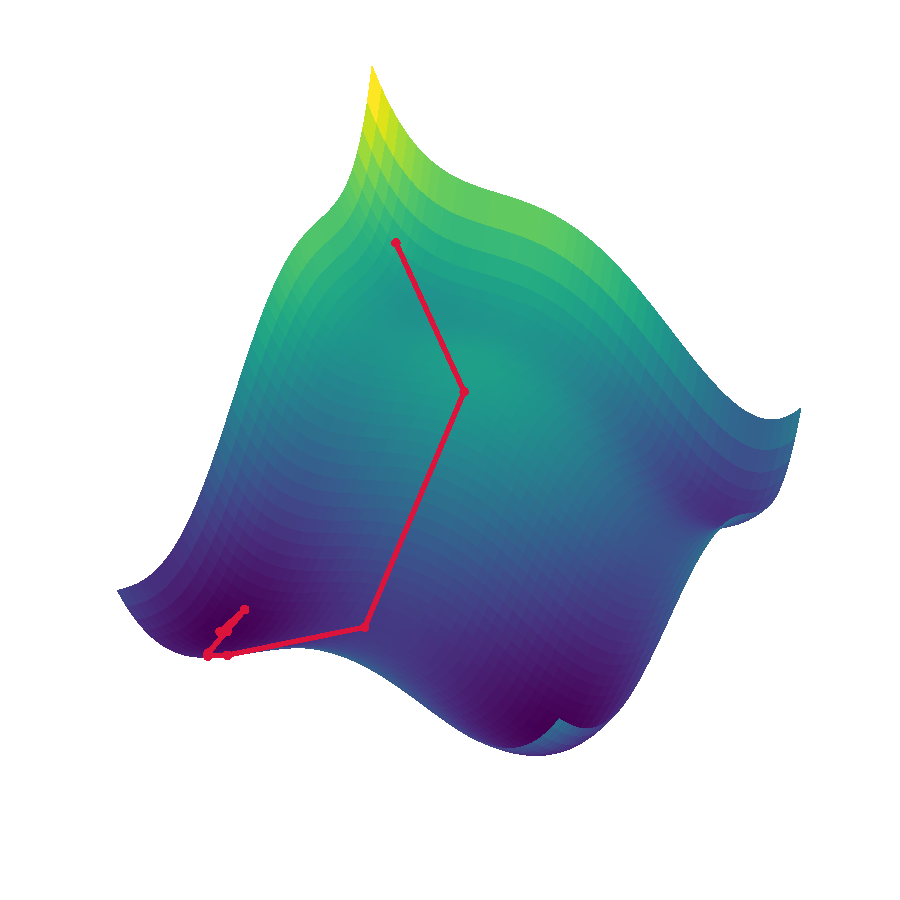
\includegraphics[height=5cm]{../imgs/quasi_newton/sixhump.pdf}
            \caption{非凸最適化の例}
        \end{minipage}%
        \begin{minipage}{0.65\columnwidth}
            \centering
            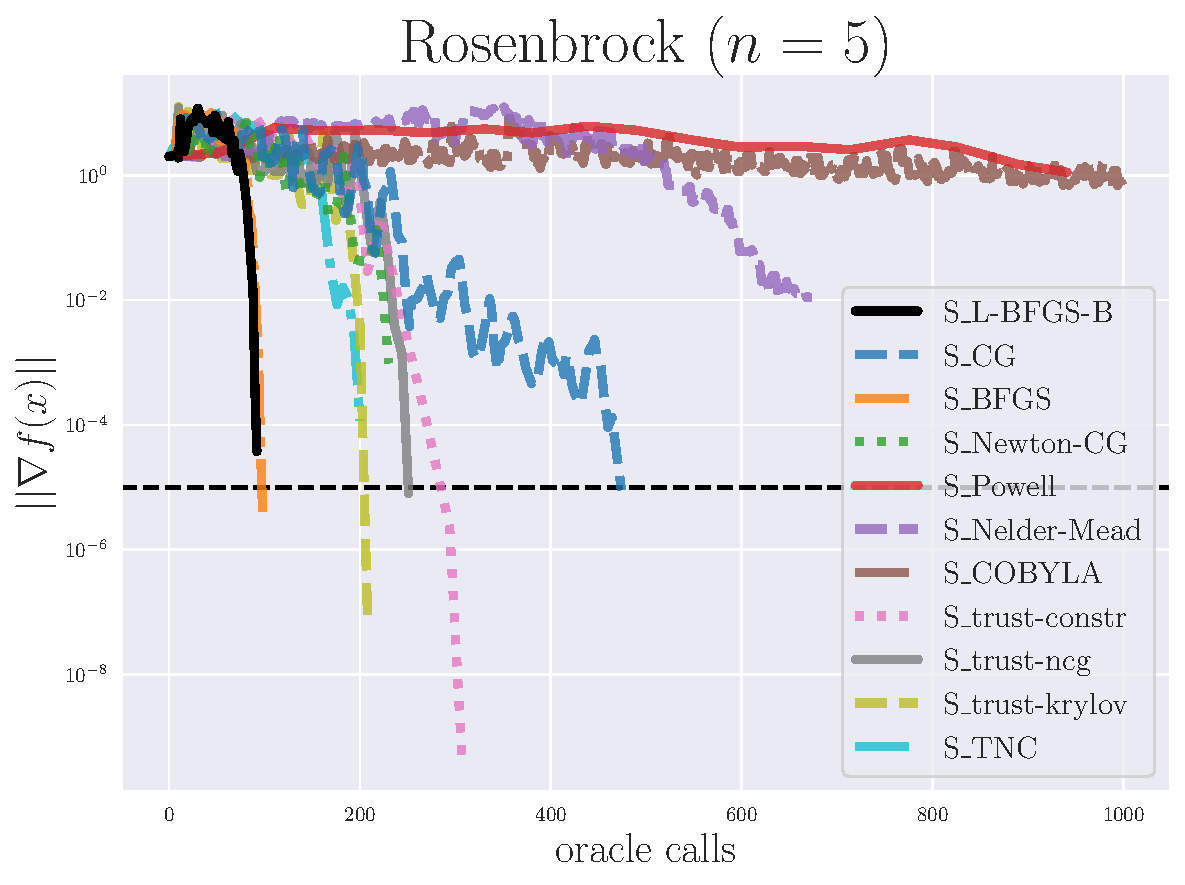
\includegraphics[height=5cm]{../imgs/quasi_newton/SciPy_comparison_Rosenbrock.pdf}
            \caption{SciPyの最適化手法の比較 準ニュートン法が最速}
        \end{minipage}
    \end{figure}
\end{frame}

\begin{frame}{問題意識: 数値誤差に対する脆弱性}
    \begin{enumerate}[label=\textbullet]
        \item 理想的な状況下で、準ニュートン法は実用上最もよく使われる手法の一つ
        \item 現実の最適化では、計算機上で行うので\textbf{数値誤差}が発生
        \item 特に、\textbf{関数値}の誤差は準ニュートン法の挙動を著しく不安定化
              \begin{enumerate}[label=--]
                  \item ビッグデータを扱う際の低精度浮動小数点数(32, 16bit)による計算や、\\
                        近似値や確率で変動する値のみが計算出来る状況では、不可避な誤差が\\
                        生じ本質的に解けない問題になる
                  \item ベンチマーク問題\citep{gouldCUTEstConstrainedUnconstrained2015}の\textbf{141/221}個が、デフォルト設定にて\\
                        先に関数値誤差が無視できないレベルで大きくなる
              \end{enumerate}
        \item 従来的な理論保証は失われ、小手先の改善では解決しない問題も多い
    \end{enumerate}
    \begin{block}{本研究の主題}
        実用的な高速性を維持しつつ、特に関数値の数値誤差に頑健な準ニュートン法とは?
    \end{block}
\end{frame}

\begin{frame}{本研究の位置づけ}
    \begin{itemize}
        \item 無視できない誤差が $f$ にも $\nabla f$ にも存在すると、その最適化問題は\colorbox{UniGray}{不良設定}
        \item 本研究は、特に\underline{関数値 $f$ の誤差が大きい場合}に着目
    \end{itemize}
    \begin{table}
        \centering
        \begin{tabular}{m{0.5cm}m{0.5cm}|C{0.4\columnwidth}C{0.4\columnwidth}}
            \toprule
             &                                                                                            & \multicolumn{2}{c}{$f$ の誤差}     \\
             &                                                                                            & 小                           & 大 \\
            \midrule
            \multirow{2}{*}{\rotatebox{90}{$\nabla f$ の誤差}}
             & \rotatebox{90}{\makebox[1.2cm][c]{小}}
             & \makecell[c]{通常の最適化                                                                                                          \\ \citep{liuLimitedMemoryBFGS1989a,2020SciPy-NMeth}}
             & \cellcolor{UniBlueLight}
            {\fbox{本研究などの対象}}
            \\
             & \rotatebox{90}{\makebox[1.2cm][c]{大}}
             & \cellcolor{UniBlueLight} \makecell[c]{先行研究\citep{shiNoiseTolerantQuasiNewtonAlgorithm2022}                                   \\(いわゆる0次法に近い手法など)}
             & \cellcolor{UniGray}(最適化不可能)                                                                                                  \\
            \bottomrule
        \end{tabular}
    \end{table}
    より緩い誤差への研究や\citep{sunTrustRegionMethod2023,paquetteStochasticLineSearch2020,byrdSampleSizeSelection2012}、\\
    信頼領域法における研究\citep{sunTrustRegionMethod2023,bellaviaImpactNoiseEvaluation2021}なども存在\\
    $\to$ 本研究は、\underline{消すことが出来ない誤差}に対して\underline{実用的な高速性を維持}したい
\end{frame}

\begin{frame}{研究概要}
    \begin{block}{本研究の主題}
        実用的な高速性を維持しつつ、特に関数値の数値誤差に頑健な準ニュートン法とは?
    \end{block}
    \begin{exampleblock}{先行研究}
        \begin{itemize}
            \item 直線探索型準ニュートン法\citep{liuLimitedMemoryBFGS1989a,2020SciPy-NMeth}は高速だが脆弱
            \item 正則化手法\citep{kanzowRegularizationLimitedMemory2023,uedaRegularizedNewtonMethod2014}は代替案として近年注目
            \item しかし、これらは数値誤差を考慮せず、また必ずしも高速ではなく、課題を残す
        \end{itemize}
    \end{exampleblock}
    \begin{alertblock}{本研究の貢献}
        \begin{itemize}
            \item 正則化準ニュートン法を用いながら、\underline{$f$ の数値誤差を陽に考慮する}
            \item 誤差問題を回避するため、$f$ を使わない\underline{関数値非依存最適化}を援用
            \item \underline{数値誤差に耐性のある高速な準ニュートン法を提案}
        \end{itemize}
    \end{alertblock}
\end{frame}

\begin{frame}{具体的な問題設定と誤差モデル}
    現実的なIEEE~754浮動小数点数を想定した誤差モデル $\overline{f}$ のみが観測可能。
    \begin{block}{関数値に対するハイブリッド型の誤差モデル}
        絶対誤差と相対誤差が混在する誤差モデル\citep{highamAccuracyStabilityNumerical2002,10.5555/3168451.3168462}:
        \begin{equation*}
            \abs{f(x)-\overline{f}(x)} \le \feps \max(1,\abs{f(x)}).
        \end{equation*}
    \end{block}
    \vspace{1em}
    停止条件は $\norm{\nabla \overline{f}(x)} \leq \gtol$ なので、過程では常に $\norm{\nabla \overline{f}(x)} > \gtol$ が成立する。
    \begin{exampleblock}{勾配に対する誤差モデル: 誤差が $\gtol$ より十分小さい}
        \begin{equation*}
            \text{(数値実験)} \norm{\nabla f(x)-\nabla\overline{f}(x)}\ll\gtol, \qquad
            \text{(理論解析)} \norm{\nabla f(x)-\nabla\overline{f}(x)}=0.
        \end{equation*}
    \end{exampleblock}
\end{frame}

\begin{frame}{キーワード:目的関数値非依存最適化 \citep{grattonOFFOMinimizationAlgorithms2023}}
    機械学習分野での需要などから近年発展してきた手法。\\
    AdaGrad や AdaGrad-Norm などの最適化手法は、勾配だけで最適化を行う。
    \begin{align*}
        (\text{AdaGrad}) \quad x_{k+1}^{(i)} & = x_k^{(i)} - \frac{1}{\theta\sqrt{\varsigma + \sum_{j=0}^k (\nabla f(x_j)^{(i)})^2}} \nabla f(x_k)^{(i)}, \\
        (\text{AdaGrad-Norm}) \quad x_{k+1}  & = x_k - \frac{1}{\theta\sqrt{\varsigma + \sum_{j=0}^k \norm{\nabla f(x_j)}^2}}\,\nabla f(x_k).
    \end{align*}
    ($\theta$ は学習率の逆数, $\varsigma$ は初期化定数, ${}^{(i)}$ は第 $i$ 成分)\\
    \vspace{2em}
    このような\underline{関数値 $f$}を陽に用いない最適化手法の総称\\
    $\to$ 誤差に影響されやすい\underline{関数値差分}を利用せずに最適化が可能に
\end{frame}

\begin{frame}{提案手法の構成要素1/2: 緩和Armijo条件}
    通常のArmijo条件 (従来的なエラーが起きる直線探索の終了条件):
    \begin{equation*}
        \overline{f}(x_k) + c \alpha_k \nabla f(x_k)^\top d_k \ge \overline{f}(x_k + \alpha_k d_k).
    \end{equation*}

    本研究は以下の緩和 Armijo 条件を採用:
    \begin{equation*}
        \begin{dcases}
            \overline{f}(x_k) + c \alpha_k \nabla f(x_k)^\top d_k + \red{\Delta_k} \ge \overline{f}(x_k + \alpha_k d_k), \\
            \red{\Delta_k} = \frac{2\feps}{1-\feps}\max(1,\overline{f}(x_k),-\overline{f}(x_k+\alpha_k d_k)).
        \end{dcases}
    \end{equation*}
    この\red{$\Delta_k$}は(適切な条件下で)次を満たす、誤差吸収項:
    \begin{equation*}
        \big| \underbrace{(\overline{f}(x_k) - \overline{f}(x_k + \alpha_k d_k))}_{\text{観測された差分}} - \underbrace{(f(x_k) - f(x_k + \alpha_k d_k))}_{\text{真の差分}} \big|
        \le \red{\Delta_k}.
    \end{equation*}
    → \underline{現実的な誤差ありの設定でも、エラーなく最適化を進められる。}
\end{frame}

\begin{frame}{提案手法の構成要素2/2: 正則化を入れた探索方向}
    探索方向は正則化付き準ニュートン方向を採用:
    \begin{equation*}
        d_k = -(B_k + \mu_k I)^{-1} \nabla f(x_k).
    \end{equation*}
    (直感: $f$ の勾配情報による近似 $B_k$ + 正則化項 $\mu_k I$ を加えた二次形式の最小解方向)
    \begin{itemize}
        \item $\mu_k=0$: 直線探索型とほぼ同じ挙動を意味、速度の観点からは望ましい
        \item $\mu_k>0$: 保守的なステップになり、安定性向上、 AdaGrad-Norm に似た正則化:
              \begin{equation*}
                  \mu_k = \theta_k \sqrt{\varsigma + \sum_{j \in K^+} \norm{\nabla f(x_j)}^2},\quad \theta_k \in [\theta_{\min}, \theta_{\max}].
              \end{equation*}
        \item $B_k \approx \nabla^2 f(x_k)$ のとき、$\mu_k > 0$ は二次近似を壊し、過度に保守的になる恐れがある。
        \item 十分に $\overline{f}$ が減少した試行では、$\mu_k=0$ を試すことで、速度と安定性の両立を図る。
    \end{itemize}
\end{frame}

\begin{frame}{本質的な設計思想の図示}
    \begin{itemize}
        \item 直線探索で $\overline{f}$ の上昇を許し、エラーを回避する(図左側)
        \item $\mu_k=0$ を優先的に試すが、十分に $\overline{f}$ が減少した試行に限ることで、安定化 (図右側)
    \end{itemize}
    \begin{figure}[htbp]
        \centering
        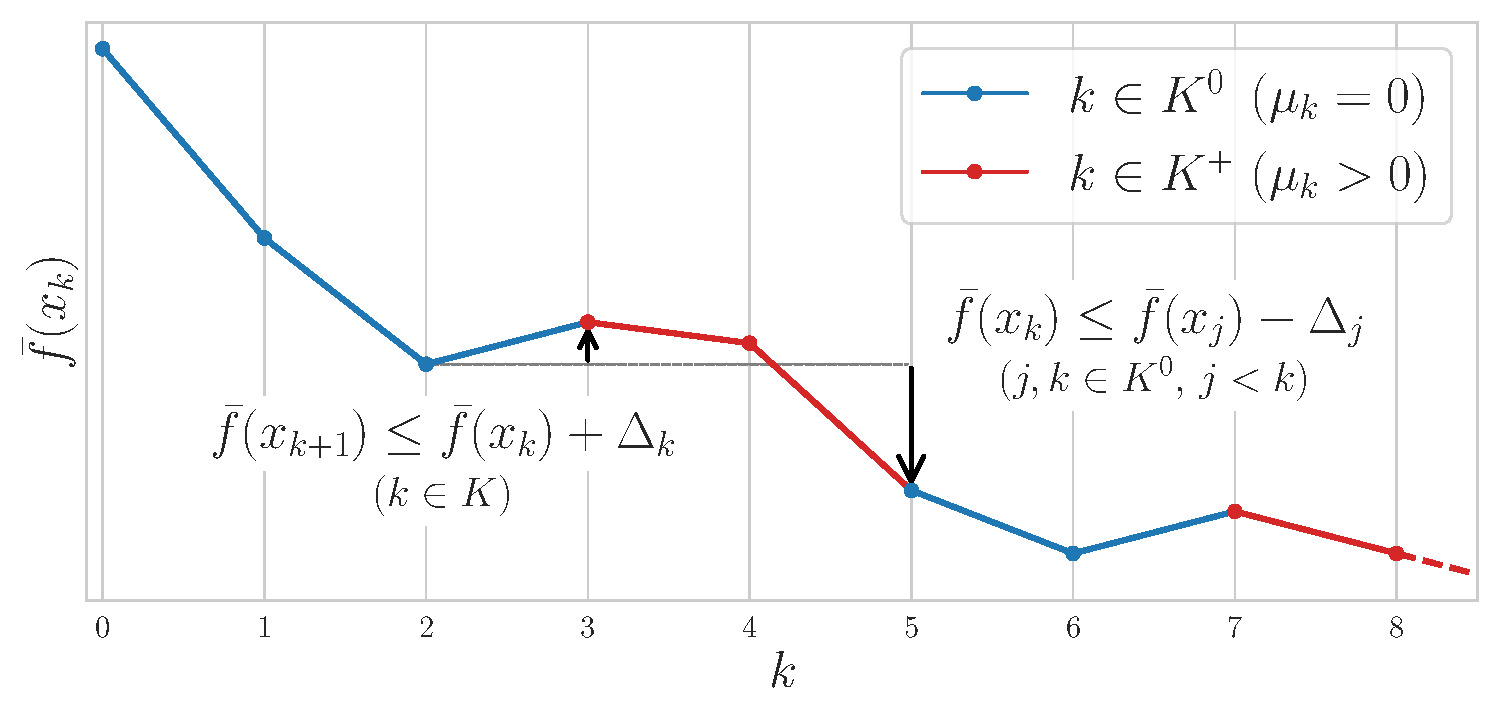
\includegraphics[width=0.8\columnwidth]{../imgs/for_paper/alg.pdf}
    \end{figure}
    \begin{equation*}
        K^0 \defeq \{k \in K \mid \mu_k = 0\}, \quad K^+ \defeq \{k \in K \mid \mu_k > 0\}.
    \end{equation*}
\end{frame}

\begin{frame}{理論解析における仮定}
    以下では、提案手法が適切な仮定の下で収束することを示す。\\[1em]

    最適化問題は、次の非常に標準的な2つの仮定を満たすとする。
    \begin{block}{仮定1: 目的関数 $f$ の下側に関する有界性}
        \begin{equation*}
            f(x) \ge f^* \defeq \inf_{x \in \bbR^n} f(x) > -\infty.
        \end{equation*}
    \end{block}
    \begin{block}{仮定2: 目的関数 $f$ の $L$-smooth性}
        \begin{equation*}
            \exists\, 0< L < \infty \quad\text{s.t.}\quad f(y) \le f(x) + \nabla f(x)^\top (y - x) + \frac{L}{2} \norm{y - x}^2.
        \end{equation*}
    \end{block}
    \vspace{1em}

    この設定の標準的な反復計算量 $\min\{k \mid \norm{\nabla f(x_k)} \le \gtol\}$ は $\Omega(\gtol^{-2})$ である。
\end{frame}

\begin{frame}{収束解析の概要: コアとなる不等式}
    \vspace{-0.7em}
    \begin{equation*}
        K^0 = \{k \in K \mid \mu_k = 0\}, \; K^+ = \{k \in K \mid \mu_k > 0\}, \; \text{(Armijo定数) }c, \; \text{(smooth性) }L.
    \end{equation*}
    \vspace{-0.7em}
    \begin{block}{勾配ノルム和に対する複合的な上界評価}
        仮定1,2の下で、
        $F = \order{f(x_0)-f^*}$,
        定数 $C_0, C_1, C_2$ を用いて\vspace{-0.5em}
        \begin{equation*}
            F \ge C_0 \sum_{k\in K^0}\norm{\nabla f(x_k)}^2 + C_1 \sqrt{\varsigma+\sum_{k\in K^+}\norm{\nabla f(x_k)}^2} - C_2\ln\Bigl(\varsigma+\sum_{k\in K^+}\norm{\nabla f(x_k)}^2\Bigr).
        \end{equation*}
    \end{block}
    \vspace{-1.2em}
    \begin{columns}[t]
        \column{0.48\textwidth}
        \begin{exampleblock}{$K^0$:正則化のない通常ステップ}
            \begin{itemize}
                \item 古典的な勾配法型の解析結果と一致:
            \end{itemize}
            \[
                \sum_{k\in K^0}\norm{\nabla f(x_k)}^2
                \lesssim \frac{1}{C_0} F.
            \]
        \end{exampleblock}
        \column{0.48\textwidth}
        \begin{exampleblock}{$K^+$:正則化が入る保守的ステップ}
            \begin{itemize}
                \item $\sqrt{\cdot} \gg \ln{\cdot}$ より、$\sqrt{\cdot}$ の項が支配的:
            \end{itemize}
            \[
                \sum_{k\in K^+}\norm{\nabla f(x_k)}^2 \lesssim \qty(\frac{2F}{C_1})^2.
            \]
        \end{exampleblock}
    \end{columns}
\end{frame}

\begin{frame}{大域収束率の結論}
    \begin{block}{主結果}
        仮定1,2の下で、任意の反復回数 $k_{\max}>0$ に対し、提案手法は以下を満たす。
        \begin{equation*}
            \sum_{j=0}^{k_{\max}-1} \norm{\nabla f(x_j)}^2 \le \text{const.}
            \implies
            \frac{1}{k_{\max}}\sum_{j=0}^{k_{\max}-1} \norm{\nabla f(x_j)}^2 = \order{\frac{1}{k_{\max}}}.
        \end{equation*}
    \end{block}
    \begin{exampleblock}{提案手法が達成する反復計算量}
        \[
            \min\{k \mid \norm{\nabla f(x_k)} \le \gtol\}
            = \order{\gtol^{-2}}.
        \]
    \end{exampleblock}
    \begin{itemize}
        \item \underline{誤差がある設定}でも、非凸問題に対する\underline{標準的な反復計算量}とオーダーレベルで一致
        \item 具体的には、古典的な勾配法型の解析結果と AdaGrad-Norm 型の解析結果\\
              のハイブリッドになっている
    \end{itemize}
\end{frame}

\begin{frame}{実験設定}
    \begin{block}{比較手法}
        \begin{itemize}[leftmargin=4em]
            \item[\texttt{Ours}:] 提案手法 (\texttt{Ours-MS} は一種の改良版)
            \item[\texttt{Line}:] Wolfe条件による直線探索型 (\texttt{Line-MS} も同様の変種)
            \item[\texttt{SciPy}:] 著名OSSである SciPy に実装された L-BFGS-B法
            \item[\texttt{Reg}:] 近年の正則化 L-BFGS法 \citep{kanzowRegularizationLimitedMemory2023}
            \item[\texttt{NTQN}:] 冒頭で述べた0次法に類似したノイズ耐性準ニュートン法 \citep{shiNoiseTolerantQuasiNewtonAlgorithm2022}
        \end{itemize}
    \end{block}
    \begin{columns}
        \begin{column}{0.4\columnwidth}
            \begin{exampleblock}{問題設定}
                \begin{itemize}
                    \item CUTEst 無制約問題
                    \item 非凸問題を含む有名ベンチマーク
                    \item 最大 220 問題
                \end{itemize}
            \end{exampleblock}
        \end{column}
        \begin{column}{0.55\columnwidth}
            \begin{exampleblock}{評価手法: Performance Profile}
                \begin{itemize}
                    \item どれだけ安定かつ高速に解けたかを評価
                    \item $x$ 軸方向に左であればあるほど高速
                    \item $y$ 軸方向に上であればあるほど安定
                \end{itemize}
            \end{exampleblock}
        \end{column}
    \end{columns}
\end{frame}

\begin{frame}{人工ノイズ下での性能}
    \begin{block}{ノイズモデル \citep{shiNoiseTolerantQuasiNewtonAlgorithm2022} ($\mathrm{unif}$ は一様分布ノイズ)}
        \[
            \overline f(x)=f(x)+\mathrm{unif}(-10^{-3},10^{-3}),\quad
            \nabla\overline f(x)=\nabla f(x)+\mathtt{unif}(-10^{-3},10^{-3}) \mathbbm{1}
        \]
    \end{block}
    \begin{columns}
        \begin{column}{0.5\columnwidth}
            \begin{center}
                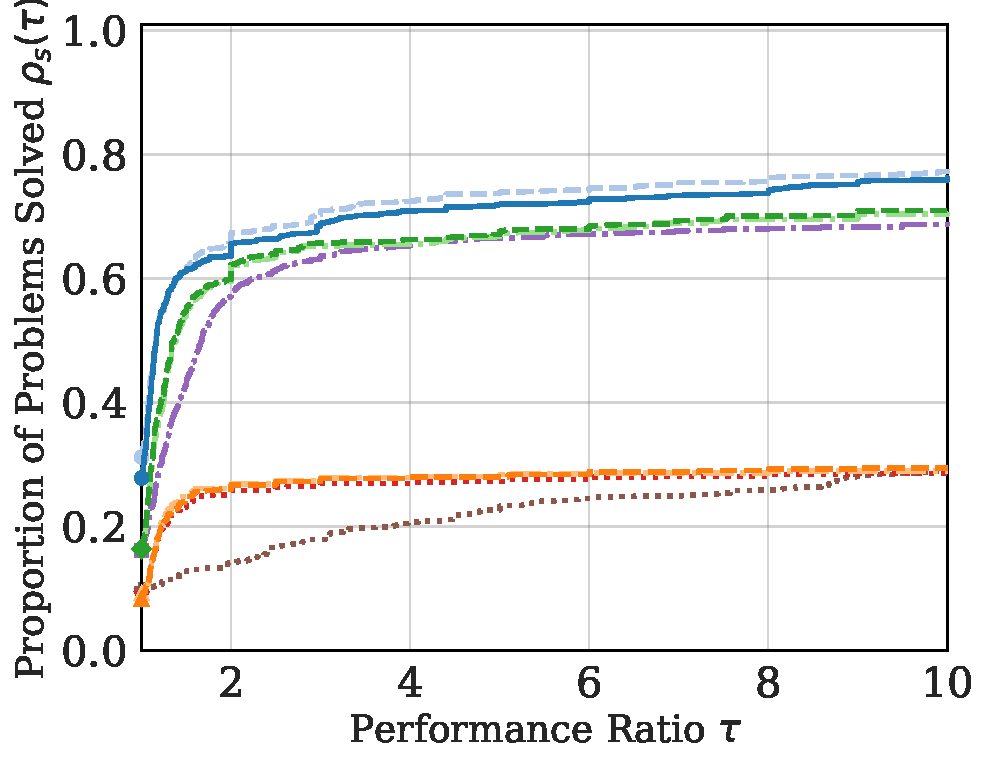
\includegraphics[width=\columnwidth]{../imgs/compare/_pp_noise0.001_gtol1e-02.pdf}
            \end{center}
        \end{column}
        \begin{column}{0.5\columnwidth}
            \begin{itemize}
                \item 提案法が最も高い成功率 \underline{(安定性)}
                \item 最速で解いた数($\tau=1$)も最多 \underline{(高速性)}
                \item 先行研究(\texttt{NTQN})\citep{shiNoiseTolerantQuasiNewtonAlgorithm2022} は勾配ノイズに特に強いアルゴリズム
                \item 我々の手法も勾配ノイズに耐性
                \item ノイズレベルを変えても同様の傾向
            \end{itemize}
            \begin{center}
                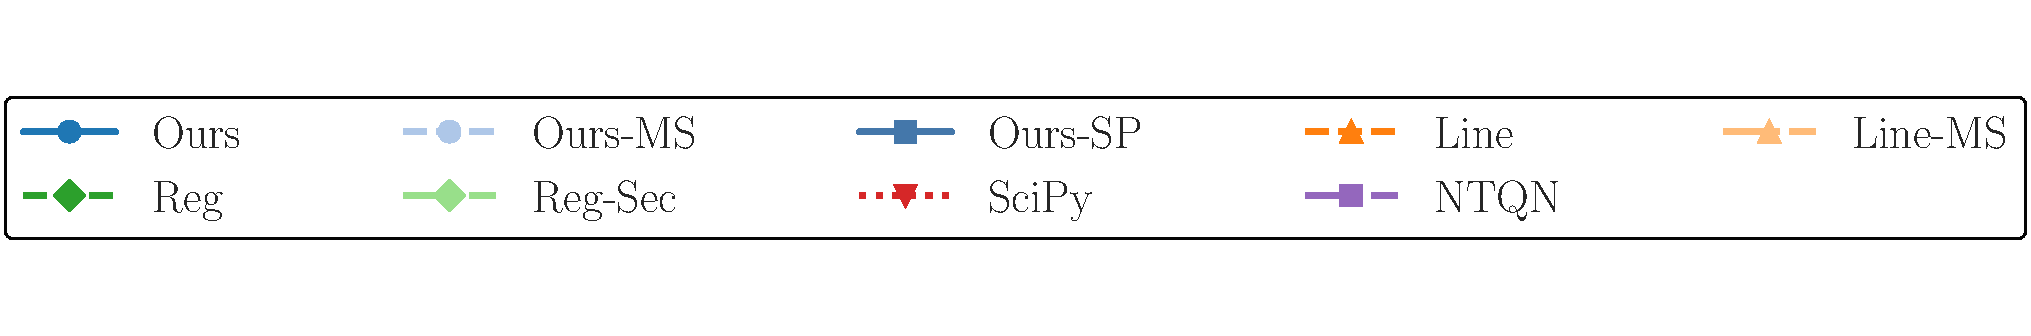
\includegraphics[width=\columnwidth]{../imgs/compare/_legend.pdf}
            \end{center}
        \end{column}
    \end{columns}
\end{frame}

\begin{frame}{有限精度計算に対する頑健性}
    \begin{columns}

        \column{0.32\textwidth}
        \centering
        64-bit $\gtol=10^{-5}$\\
        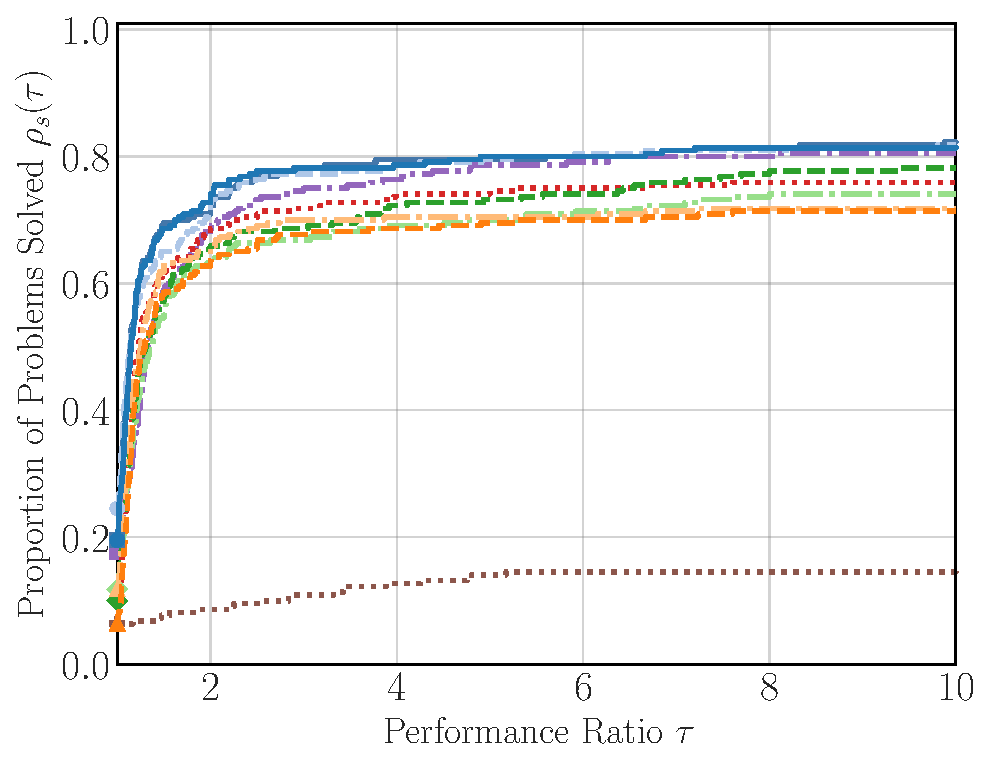
\includegraphics[width=\linewidth]{../imgs/compare/_pp_precision64_gtol1e-05.pdf}

        \column{0.32\textwidth}
        \centering
        32-bit $\gtol=10^{-4}$\\
        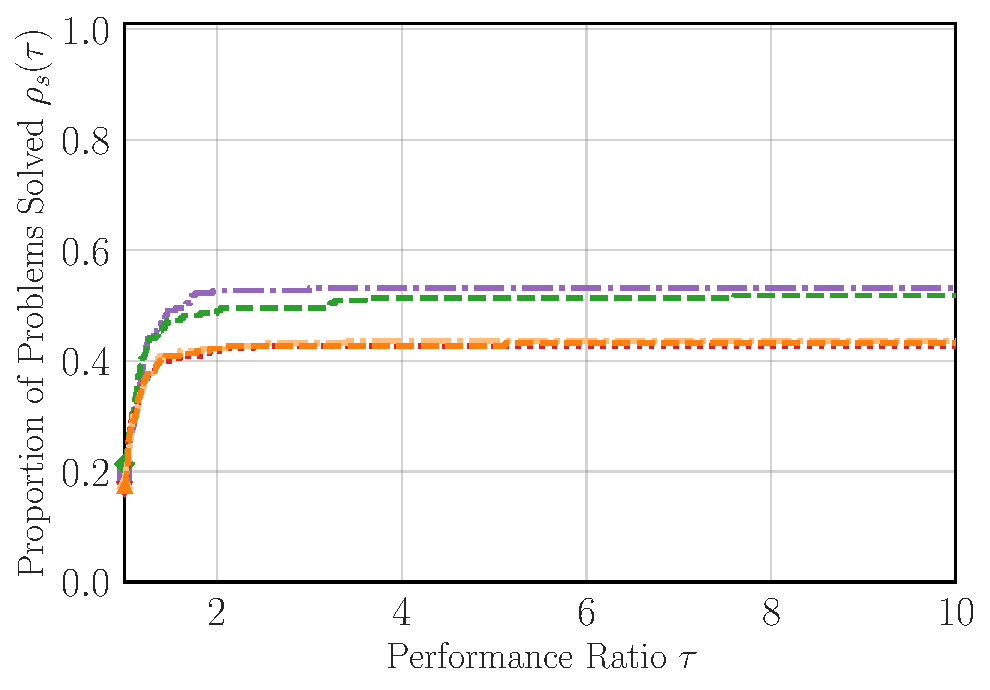
\includegraphics[width=\linewidth]{../imgs/compare/_pp_precision32_gtol1e-04.pdf}

        \column{0.32\textwidth}
        \centering
        16-bit $\gtol=10^{-3}$\\
        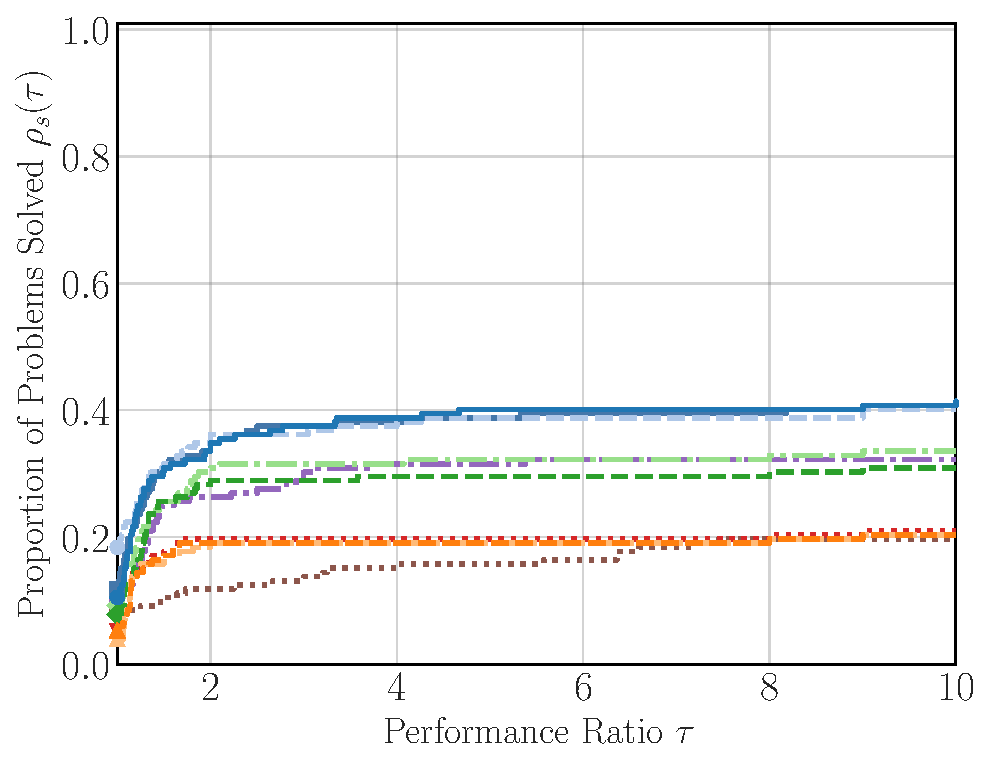
\includegraphics[width=\linewidth]{../imgs/compare/_pp_precision16_gtol1e-03.pdf}

    \end{columns}

    \begin{center}
        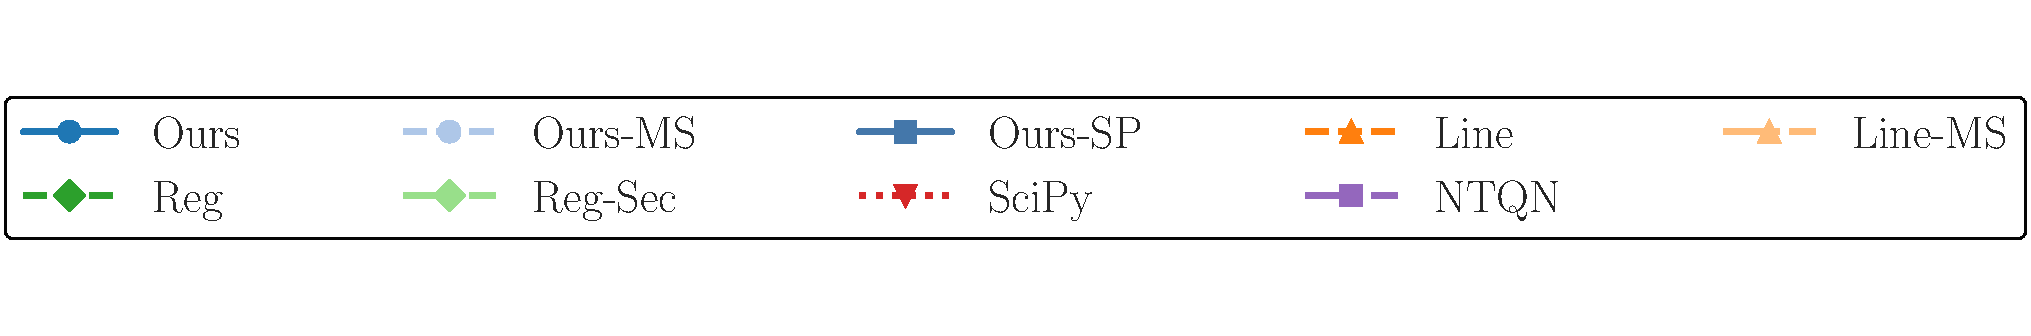
\includegraphics[width=0.8\columnwidth]{../imgs/compare/_legend.pdf}
    \end{center}

    精度低下に伴い既存法は不安定化 提案手法(\texttt{Ours})は一貫して高い成功率

\end{frame}

\begin{frame}{誤差なし設定からみる実用性}
    \begin{columns}
        \column{0.35\textwidth}
        \begin{center}
            誤差の殆ど関係ない設定:\\
            64-bit $\gtol=10^{-3}$\\
            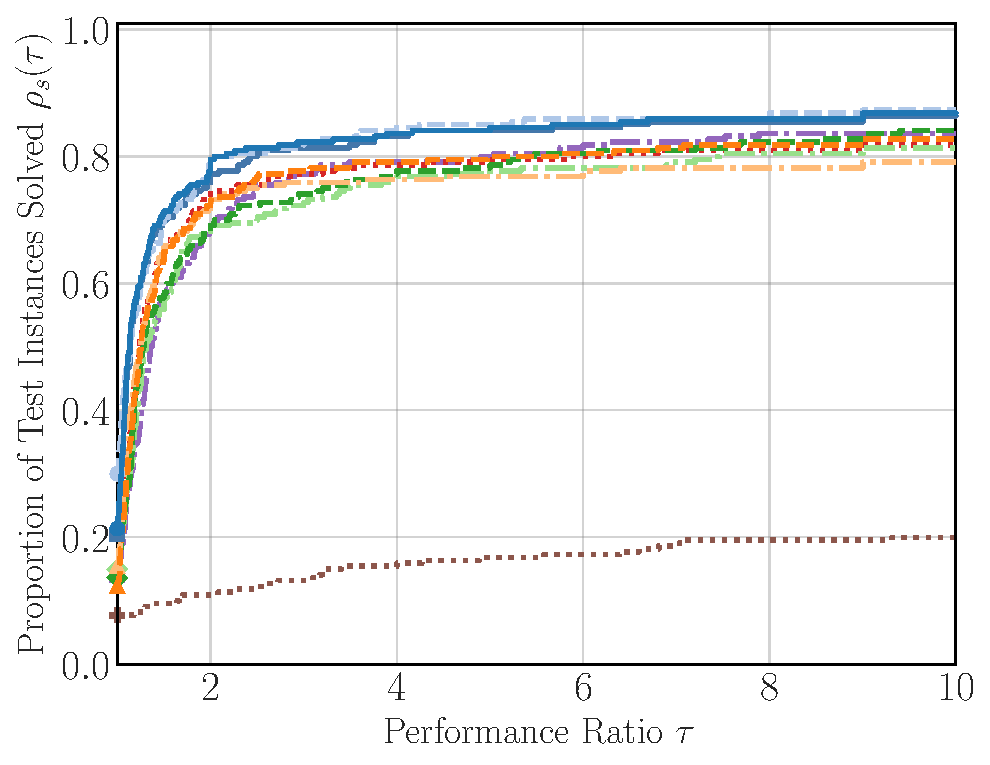
\includegraphics[width=\columnwidth]{../imgs/compare/_pp_precision64_gtol1e-03.pdf}
            最速で解けた問題数が、\\
            2倍近くに達している
        \end{center}
        \hfill
        \column{0.65\textwidth}
        \begin{itemize}
            \item 提案手法は誤差なし設定でも高速
            \item (最速で解けている問題数がSciPyの約2倍)
            \item {}
            \item 既存の理論的に良い正則化に類似点 $(c_1, c_2, \delta > 0)$:
                  \begin{equation*}
                      \mu_k ={}   c_1 \max(0, -\lambda_{\min}(B_k)) + c_2 \norm{\nabla f(x_k)}^\delta.
                  \end{equation*}
            \item {}
            \item 近似ヘッセ行列 $B_k$ に既存の工夫も活用:
                  \begin{equation*}
                      \mathrm{BFGS}(\{(s_{k_i}, \overline{y}_{k_i} \defeq \theta^{\mathrm{damp}}_i y_{k_i} + (1-\theta^{\mathrm{damp}}_i) B_{k-1}s_{k_i})\}).
                  \end{equation*}
                  ($\mathrm{BFGS}(\cdot)$ は更新則の関数、$s_{k_i}, y_{k_i}$ は差分ベクトル)
        \end{itemize}
    \end{columns}
\end{frame}

\begin{frame}{実行時間からみる実用性}
    \begin{columns}
        \column{0.6\textwidth}
        \begin{center}
            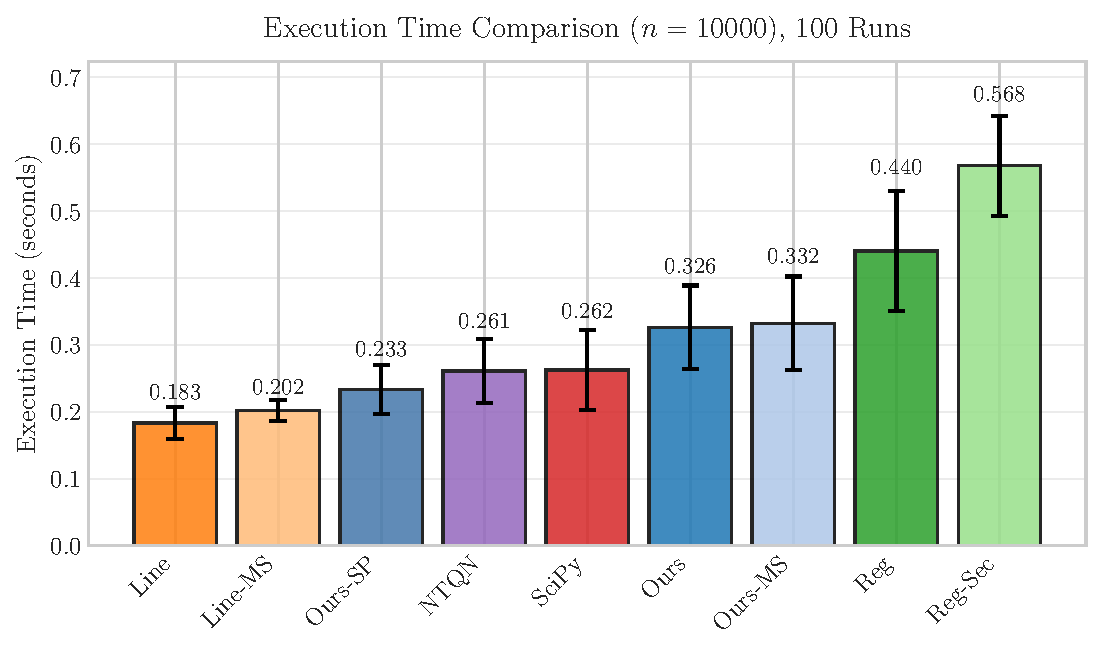
\includegraphics[width=\columnwidth]{../imgs/for_paper/time.pdf}
        \end{center}
        \column{0.4\textwidth}
        \begin{itemize}
            \item 左図は大まかにアルゴリズム自体 ($f$ や $\nabla f$ を除く) の計算時間。
            \item 正則化型の手法
                  \begin{equation*}
                      d_k =-(B_k+\mu_k I)^{-1}\nabla f(x_k)
                  \end{equation*}
                  は行列計算に時間を要する。
            \item 提案は既存の近似手法を採用。
            \item それでも性能は落ちない。
        \end{itemize}
    \end{columns}
    \begin{align*}
        \text{(近似ヘッセ行列)} &  & B_k & \approx\mathrm{BFGS}(\{s_{k_i},\overline{y}_{k_i}+\mu_k s_{k_i}\}_{i=0}^{p-1})-\mu_k I, \\
        \text{(探索方向)}    &  & d_k & =-(B_k+\mu_k I)^{-1}\nabla f(x_k) = -\mathrm{BFGS}(\dots)^{-1}\nabla f(x_k).
    \end{align*}
\end{frame}

\begin{frame}{余談: 修士1年での研究内容との関連}
    \begin{columns}
        \column{0.45\textwidth}
        \centering
        研究概要図\\
        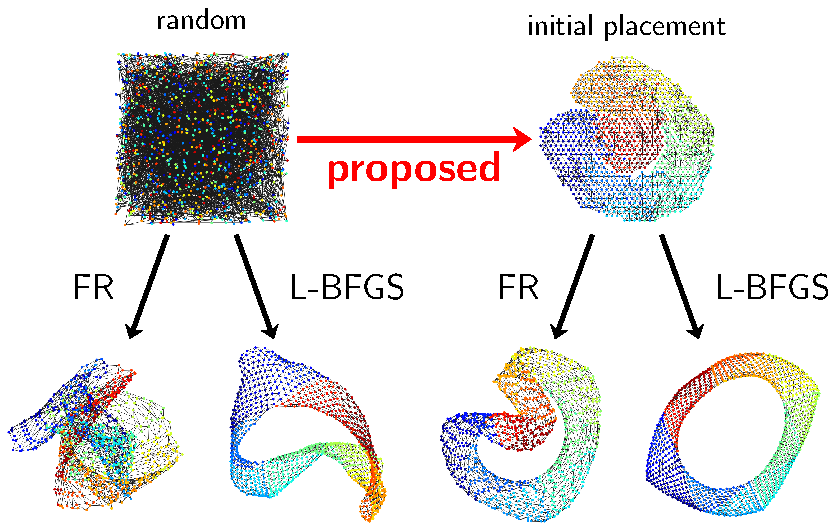
\includegraphics[width=\linewidth]{../imgs/fig1_slide.pdf}
        \column{0.45\textwidth}
        \centering
        NetworkXへ果たした貢献\\
        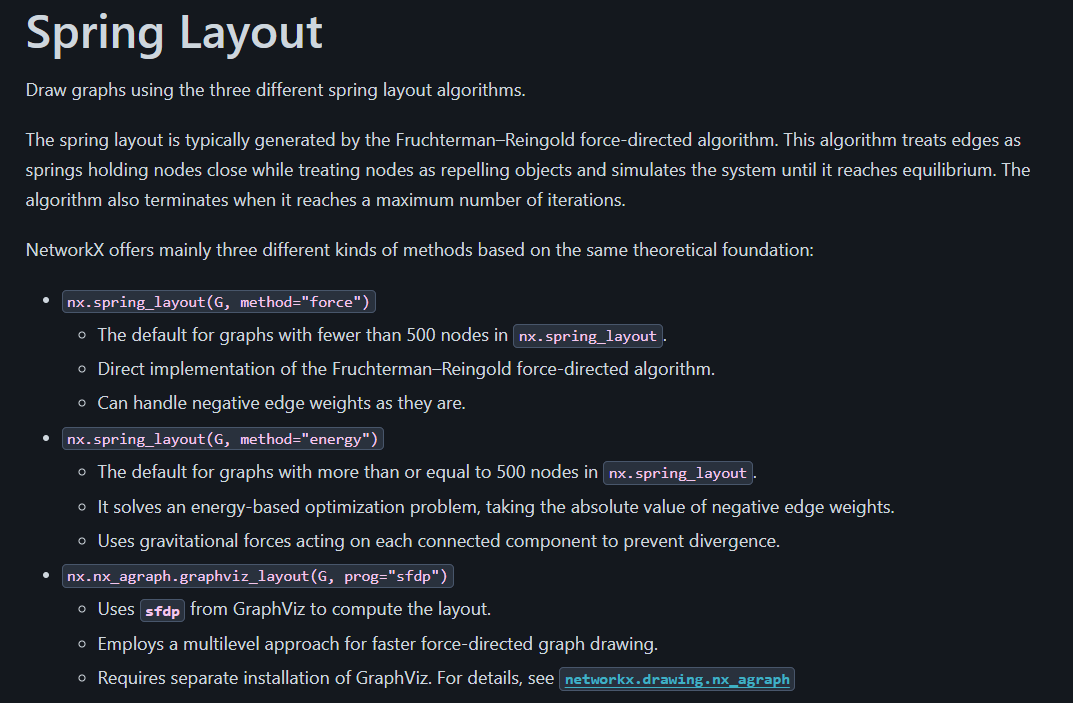
\includegraphics[width=\linewidth]{../imgs/NetworkX.png}
    \end{columns}
    \begin{itemize}
        \item 連続最適化を用いたグラフ描画の研究:
        \item {\small ``Initial Placement for Fruchterman--Reingold Force Model with Coordinate Newton Direction''}
        \item L-BFGS法は、そのグラフ描画においても高速で有用な手法。
        \item NetworkXに関連した実装を行い、\texttt{nx.draw}関数を改善。
        \item SciPyにも似たような貢献が出来ればと考えている。
    \end{itemize}
\end{frame}

\begin{frame}{まとめと今後の課題}
    \begin{block}{まとめ}
        \begin{itemize}
            \item 数値誤差を陽に考慮した正則化付き準ニュートン法を提案
            \item 緩和Armijo条件により関数値誤差を吸収し安全に更新
            \item 正則化パラメータ $\mu_k=0$ と $\mu_k>0$ の切替で高速性と安定性を両立
            \item 標準仮定の下で、非凸における最適レートと同じオーダーの収束率 $\order{\epsilon^{-2}}$ を証明
            \item 既存の人工設定 + 有限精度環境のCUTEstデータセットで安定性と高速性を確認
        \end{itemize}
    \end{block}
    \begin{exampleblock}{今後の課題}
        \begin{itemize}
            \item 勾配にも無視できない誤差がある場合との統合、理論解析の強化
        \end{itemize}
    \end{exampleblock}
\end{frame}

\appendix

\setbeamercolor{structure}{fg=black!80}
\setbeamercolor{block title}{fg=black!80}

\newcommand{\backupbegin}{
    \newcounter{framenumberappendix}
    \setcounter{framenumberappendix}{\value{framenumber}}
}
\newcommand{\backupend}{
    \addtocounter{framenumberappendix}{-\value{framenumber}}
    \addtocounter{framenumber}{\value{framenumberappendix}}
}

\backupbegin

\begin{frame}[allowframebreaks]{Reference}
    \scriptsize
    \beamertemplatetextbibitems
    \bibliographystyle{plainnat}
    \bibliography{../L-BFGS}
\end{frame}

\backupend

\end{document}